\chapter{Model Analysis}

\epigraph{The more we play cricket, the more players will learn from it}{Inzamam-ul-Haq}

This chapter is dedicated to analysing the results of the neural network model implemented in the prior chapter. We first look at how the model did on predicting the test dataset 
that is in exactly the same form as the training data. We then give a brief mathematical interlude on Monte-Carlo simmulation before using this to create a simmulated dataset 
to test the model on. Finally, we give the network actual DLS game data to see how it does. In each of the cases, we perform similar analysis to compare the performance of the model.
The main metric is the corrolation between actual results and those predicted by the network.

\section{Fully trained Neural Network}
The first thing to look for is the normality of the errors in the predicted values. If the errors are normally distrubted (and ideally around 0),
then it means that our predictions are sufficiently accurate. We produce a density plot of the errors using the \textit{ggplot2} library in R.

\begin{figure}[h]
    \centering
    \subfloat[\centering Distribution of Errors]{{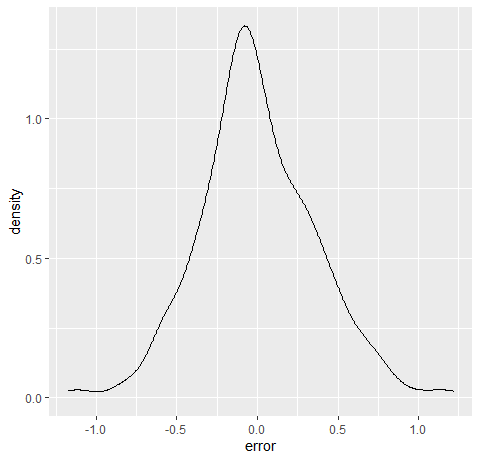
\includegraphics[width=.4\linewidth]{figures/errDist.png} }}
    \qquad
    \subfloat[\centering Q-Q Plot of Errors]{{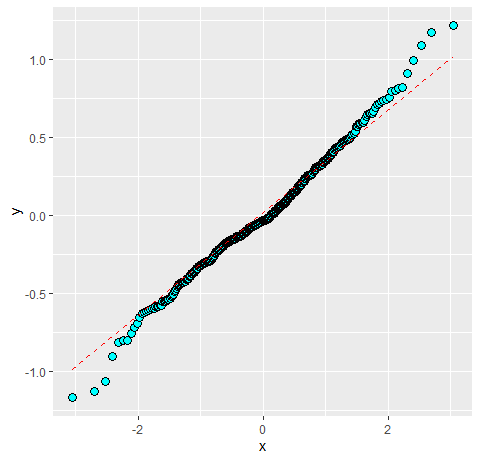
\includegraphics[width=.4\linewidth]{figures/errorqq.png} }}
    \caption{Error distribution with Q-Q plot}
    \label{errDistAndQQ}
\end{figure}

As we can see in this figure, there is a general bell curve, but not quite perfect as we have a bump between -0.5 and -0.75, as well as between 0.125 and 0.5. This 
non-normality is reflected in the Q-Q plot of the error. Measuring accuracy of the results is harder for these value prediction networks is harder than in classification 
problems. This is because we can't construct a prediction matrix. We don't expect the network to predict values down to the exact run, this would require a lot more 
data than is available, and a large amount of experimentation. One metric we can therefore use to see how accurate our model is, is to calculate 
the corrolation between the actual results and the predicted results. Using the inbuilt \textit{cor()} function, we obtain a corrolation value of 
$0.9382$. Given how close this is to 1, which would be perfect corrolation, it is fair to say that this method has done well to predict scores. \\

The issue that one may point out here is that this network has been trained on a full-over dataset, and then been tested on a full-over dataset. But the purpose of this 
investigation has been to look at the scenario in which a full game has been completed. So the method is currently ineffective at doing the task it set out to solve. For this reason,
we must come up with a way to 'fill in' the missing overs. The idea for this is to use Monte-Carlo simmulation. We discussed in \ref{exprr} how depending on the stage of the game,
the runrates can be drawn from one of three normal distributions. So for the overs that are missed, we can simply fill in the gaps by drawing a value from the distribution that the missing over falls 
into. 

\section{Interlude: Monte-Carlo Simmulation}
\label{mcsim}
Before simmulating cricket games to test our network on, we first find it necessary to delve into the mathematics of the methods used to for doing the simmulating. This is where
``Monte-Carlo'' simmulating comes in. \\
Let H be some random variable. At this stage, the distribution of H is irrelevant, but we note that $\mu = E(H)$. Formally, we have the following definition.

\begin{definition}
    Let $n \in \mathbb{N}$ and let $\{H_i \ | \ i =1,\ldots,n\}$ be i.i.d copies of H. The \textbf{Monte-Carlo Estimate} of $\mu$, is given as $\hat{\mu}=\frac{1}{n}\sum_{i=1}^n H_i$.  
\end{definition}

Recall the well-known \textit{Strong Law of Large Numbers}.

\begin{theorem}
    \label{slln}
    Let $n \in \mathbb{N}$, and let $H_1$,$H_2$,... be an i.i.d sample from a distribution with expectation $\mu$ and standard deviation $\sigma$, with $\mu, \ \sigma < \infty$.
    Then 
    $$ 
        P\left( \lim_{n \to \infty} \bar{H}_n = \mu \right) = 1
    $$
\end{theorem}

It follows from Theorem \ref{slln} that

\begin{align}
\lim_{n \to \infty} \hat{\mu} &= \lim_{n \to \infty} \frac{1}{n}\sum_{i=1}^nH_i \\
                              &= E(H) \\
                              &= \mu.
\end{align}

\section{Match Simulation}
With the theoretical framework for Monte-Carlo simmulation established, we can now look to build an algorithm for simmulating cricket matches. Based on our own work in Chapter 4, 
we begin by defining three random variables, $R_{\text{powerplay}} \sim N(\mu_{\text{powerplay}},\sigma_\text{powerplay})$, $R_{\text{middle}} \sim N(\mu_{\text{middle}},\sigma_{\text{middle}})$
and $R_{\text{final}} \sim N(\mu_{\text{final}},\sigma_{\text{final}})$.

The numerical values for these are given in the following table.

\begin{table}[h]
    \centering
    \begin{tabular}{c | c | c}
        Numerical Values & $\mu$ & $\sigma$ \\
        \hline
        $R_{powerplay}$ & 1.5298 & 0.4486 \\
        $R_{middle}$ & 1.6541 & 0.3355 \\
        $R_{final}$ & 3.1493 & 1.1349 
    \end{tabular}
    \caption{Numerical values of the parameters used for Monte-Carlo simmulation}
\end{table}

The code for doing this simmulation was not hard to write, and after a few small performance enhancements ran almost instantaneously. The code can be seen in figure \ref{mcecode}.

\begin{figure}[h] %MAKE SURE THESE ARE THE RIGHT LINES OF CODE!!
    \label{mcecode}
    \lstinputlisting[language=R, firstline=5,lastline=25]{../code/PyScripts/monteCarlo.py}
    \caption{Implementing a Monte-Carlo Simmulation fo Cricket Matches}
\end{figure}

It is best to think of n as a sort of fine-tuning parameter. If we have n too large, we would simply be simmulating the average cricket game, while have n too low and 
we are open to having an outlier. As for the other parameters, we have \textit{overs} being the number of overs in the game, and \textit{state} determines the over to start 
simmulating from. So if we want to simmulate the whole game, set $state=1$ and $overs=50$. The array \textit{runrates} just holds the data.\\

We then have the function \textit{MCE(n,state)}. The first line of this is a ``Ternary Operator'' to determine a parameter $t$. The job of $t$ is to be an index which obtains 
the correct parameters from the arrays in lines 2 and 3. This is then fed into the next line, uses the \textit{random.normalvariate()} function to populate an empty list with random 
values drawn fro the appropriate distribution of R. This is then averaged and returned by the function. Completing the main part of the Monte-Carlo method.
Finally, a while-loop runs through the overs needed and adds the estimation values to the \textit{runrates} array. \\

To give an idea of how the value of $n$ affects the resulting simmulation, we ran two simulations, using a small value $n=5$, and a larger one using $n=100$. 

\begin{figure}[h]
    \centering
    \subfloat[\centering $n=5$]{{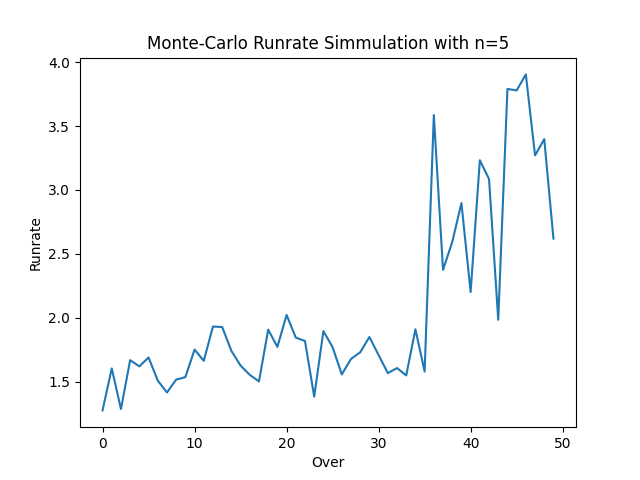
\includegraphics[width=.4\linewidth]{figures/mcen5.png} }}
    \qquad
    \subfloat[\centering $n=100$]{{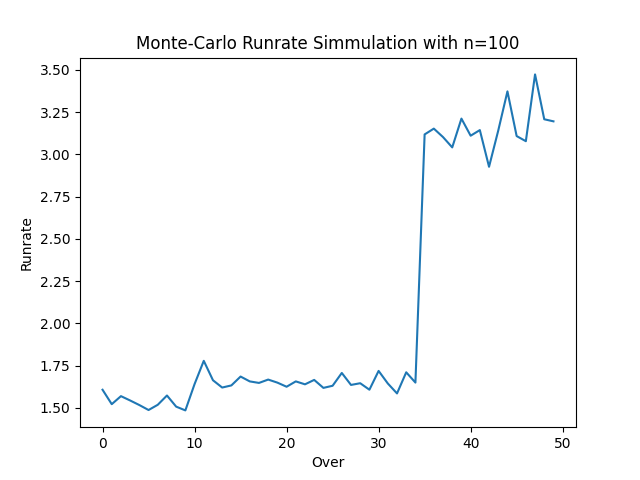
\includegraphics[width=.4\linewidth]{figures/mcen100.png} }}
    \caption{50-Over simmulation of $n=5$ and $n=100$}
    \label{MeanAndSDRR}
\end{figure}

If we compare these figues with (a) in Figure \ref{MeanAndSDRR}, we see that with large $n$, we have fallen victim to the ``Central-Limit Theorem'', and it looks as if the three 
sections of the game are unrelated. In the end, $n=20$ was the chosen value as it provided an appropriate middleground. \\

Testing if Monte-Carlo simmulation works was done in R by first cutting off each game in the original test set and random points, filling the rest in using the Monte-Carlo algorithm 
as previously described, and then feeding this into the neural network we built in the prior chapters. 

\begin{figure}[h]
    \centering
    \subfloat[\centering Error in Predictions from Monte-Carlo Simmulation]{{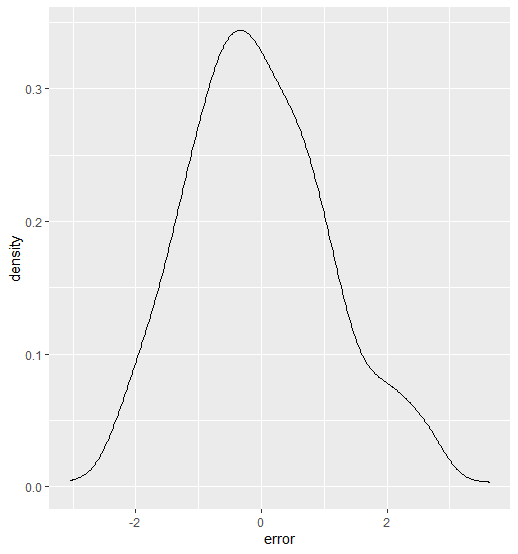
\includegraphics[width=.4\linewidth]{figures/monteCarloSimError.png} }}
    \qquad
    \subfloat[\centering Q-Q Plot of Monte-Carlo Prediction Errors]{{\includegraphics[width=.4\linewidth]{figures/monteCarloErrorQQ.png} }}
    \caption{Monte-Carlo Simmulation Error Density}
    \label{mcerror}
\end{figure}

Up until an error of around 2, we see this was more normally distributed than the original predictions. It is worth noting that this could be a side-effect of the fact that during the monte-carlo 
simmulation, all the games are being drawn directly from a normal distribution. To see definatively how the model compares to the neural network with full data, we take the corrolation of the actual results with those of the predicted values. 
We find that $\rho_{Network} = 0.9382$ and $\rho_{Monte-Carlo} = -0.0636$. So we see that when filling in the gaps with monte-carlo methods, the performance drops significantly. To further see this difference in performance, 
we calculate the difference of the monte-carlo method predictions and the original predictions, and take a boxplot.

\begin{figure}[h]
    \centering
    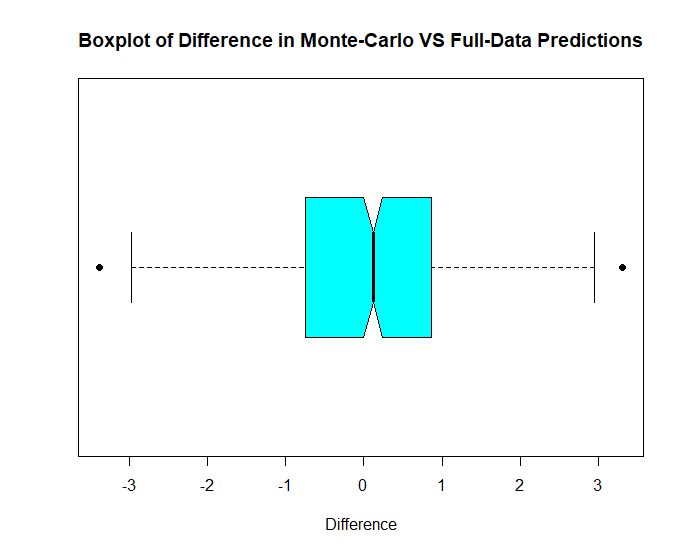
\includegraphics[width=0.4\linewidth]{figures/diffbox.png}
    \caption{Boxplot of prediction differences}
    \label{diffbox}
\end{figure}

We can see in Figure~\ref{diffbox}, that the difference is mostly centered around 0, which is promising, but the fact the corrolations are close to 0 means this is not a reliable method for predicting 
cricket scores. This is clearly an issue, because when it comes to resetting scores, the game obviously wont have a full 50 overs played, and so we need to fill in the gaps. We can then decrease the target score in proportion 
with the number of overs lost.

To put these results in more context, the data must be unscaled. The data was originally scaled using the base-R function \textit{scale()}. This applies the function

\[
    x_{\text{scaled}} = \frac{x_{\text{original}}-\mu}{\sigma}.    
\]

The parameters in the scaling can be re-obtained in R using the \textit{attr()} function. So implementing a function that 
performs unscaling on a new dataset is not too difficult, and can be achieved in afew lines of code. Note that the value of 51 has been hardcoded 
here as this is the column in which the runs scored are stored, but to make this more general, that value could be assigned dynamically.

\begin{figure}[h]
    \lstinputlisting[language=R, firstline=56,lastline=64]{../Code/Rscripts/monteCarlo.R}
    \caption{R function for unscaling data}
    \label{unscale}
\end{figure}

The function allows us to then see the actual predicted runs from both the complete neural network, and the neural network with 
gaps filled in via the Monte-Carlo method. Once this is done, for each game in the test set we plot the actual score, the score predicted by the full neural network and 
the score as predicted via the monte-carlo method. 

\begin{figure}[h]
    \label{fullPredDist}
    \centering
    \caption{Plot of predictions for all methods}
    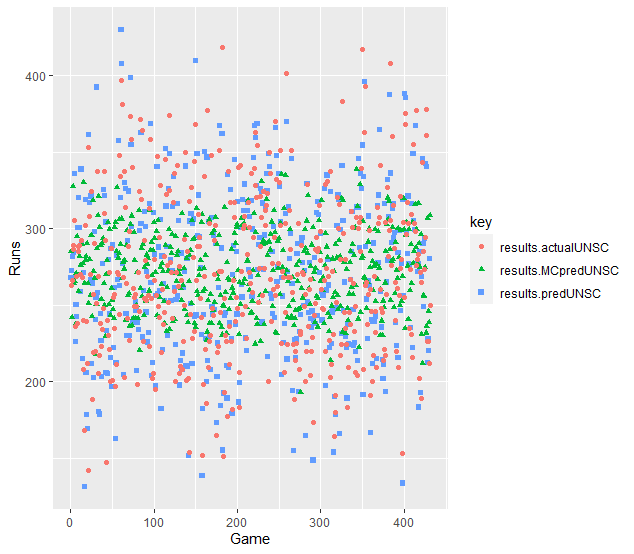
\includegraphics[scale=0.6]{figures/fullPredDist.png}
\end{figure}

This plot is naturally very busy, and it wont be used for detailed analysis of the accuracy, but what it does do well is give an overarching picture of the predictions. 
We can see that while the spread of red (actual scores) and blue (full network predictions) aren't too dissimilar, the spread of green points (monte-carlo predictions) is small and centered mainly 
around average game scores. This explains the poor performance of the model, it doesn't fair well with games that deviate far from the average. It is natural to ask how we can fix this. The one way that 
could lead to higher performance is to shrink the game into smaller chunks. Rather than looking at the three meta-stages of the game as we did originally, what about drawing from distributions of every 5 or 10 overs.

\section{Unseen DLS Game Data}
Since using Monte-Carlo methods didn't work too well, the next step is to look at seeing if something simpler will work. To do this, we take games that were decided through DLS, and 
feed them into the network to see how well it does. Rather than filling in the blanks of overs not played, we just set the runrate to 0 in these overs, and feed the resulting games into the neural network. 
We took 51 games which were decided by DLS, and looked at what the target set by DLS was. 

The results for this were actually better than for the monte carlo gap filling method. We achieved a corrolation in the results of 0.4983. Which is naturally lower than we would like, but a large improvement 
on the prior method. We can see in Figure~\ref{DLSError} how the spread of points isn't in a narrow band as it was with monte carlo predictions. We can also see the errors that came along with the predictions.

\begin{figure}[h]
    \centering
    \subfloat[\centering Network predictions for DLS games]{{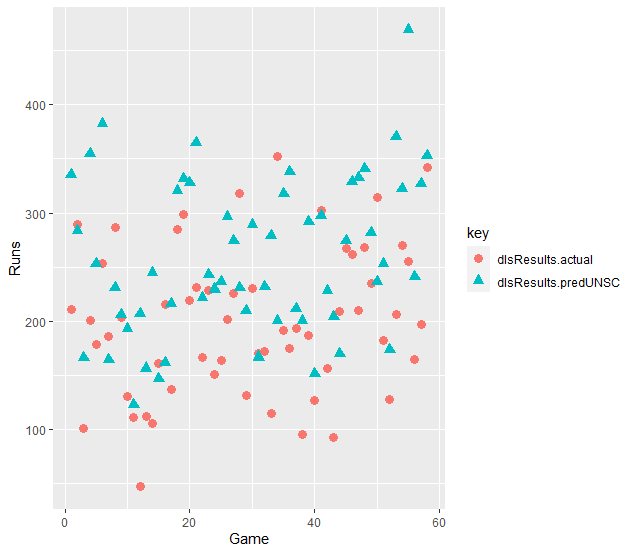
\includegraphics[width=.4\linewidth]{figures/dlsPreds.png} }}
    \qquad
    \subfloat[\centering DLS Prediction Errors]{{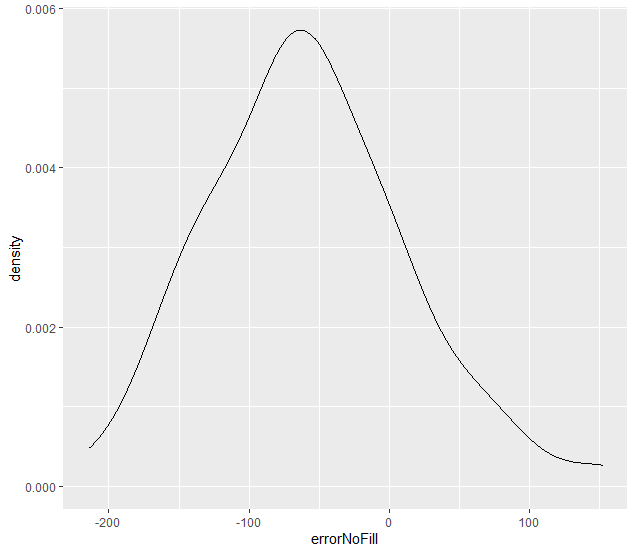
\includegraphics[width=.4\linewidth]{figures/dlsErrorDist.png} }}
    \caption{Monte-Carlo Simmulation Error Density}
    \label{DLSError}
\end{figure}


These errors are follow a rough bell-curve shape, however we must remember that there aren't many datapoints here, so it may well be that with more datapoints, we would see more of a normal distribution. The downside however is 
that this curve is not centered around an error of 0, but around -58.22. This means that on average, the model sets teams a target of a much higher score. 

